\documentclass[10pt]{article}
\usepackage[T1]{fontenc}
\usepackage{lmodern,amsmath,amssymb,graphicx,hyperref}
\usepackage[margin=.75in]{geometry}
\setlength{\parindent}{0pt}\setlength{\parskip}{6pt}
\begin{document}
\begin{center}{\Large The actual cubic helper has nonzero norm}\\[3pt]
23 November 2026 --- local unsigned Lean evidence\end{center}
\textbf{Actual construction.} For the original coefficient embedding $E(v)$,
let $A=\operatorname{evenPart}(f,v)$ and $B=\operatorname{oddPart}(f,v)$.
The accepted exact monic remainder is $A+BY$. Define $N=A^2-fB^2$.
Over a field, if $\deg f=3$ and the actual curve remainder is nonzero,
then $N\ne0$. No favorable norm or nonsquare witness is assumed
(PCC-20261123-ecff13) [pcc:unverified].

\textbf{Proof.} If $N=0$, then $A^2=fB^2$. If $B=0$, reducedness gives
$A=0$, contradicting the actual remainder. If $B\ne0$, the cubic and
$B^2$ are nonzero, so exact polynomial degrees give
$2\deg A=3+2\deg B$, impossible by parity.
The earlier actual bounds $\deg A\le15$, $\deg B\le13$ also give
$\deg N\le\max(30,3+26)=30$, including zero coefficients.
This reuses standard polynomial degree algebra [pcc:unverified].

\begin{center}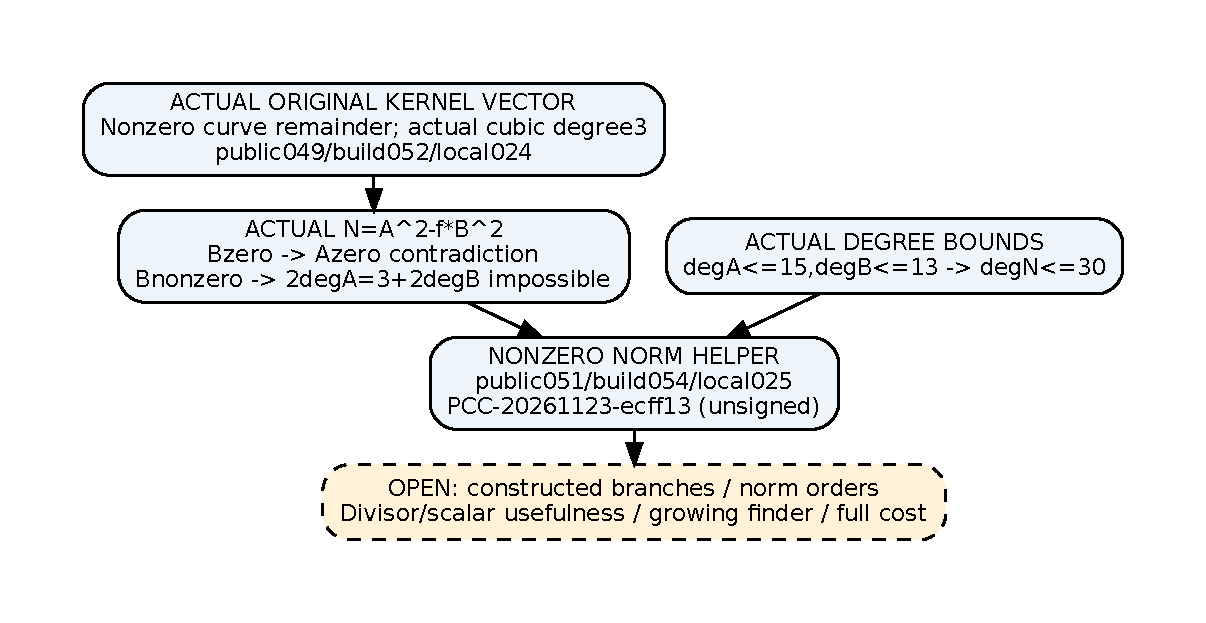
\includegraphics[width=.76\linewidth,height=.34\textheight,keepaspectratio]{norm-dependencies-001.pdf}\end{center}
\textbf{Exact scope.} Existing actual nonzero remainder image supplies a
vector in the original interpolation kernel with $N\ne0$ and
$\deg N\le30$. The curve-point assumptions remain explicit:
three paired abscissas, distinct singleton target, actual node equivalence,
$2\ne0$, nonzero ordinates and $y^2=f(x)$; the norm corollary strengthens
$\deg f\le3$ to $\deg f=3$ [pcc:unverified].

\textbf{Proof map and checks.}
Namespace \texttt{OrientationActualCubicNorm}:\par
\texttt{actualNorm\_nonzero},
\texttt{actualNorm\_degree}, and
\texttt{actual\_nonzero\_norm\_helper}.\par
Source 051, build 054, receipt 025: three new statements, 129 including 126 parent;
exit zero, no warnings, all 129 printed dependencies standard.
Failed source 050, build 053 used a nonexistent lemma name; 051 uses the exact
public \texttt{eq\_zero\_of\_pow\_eq\_zero} law. Both sources/raw logs/exits
are retained. Lean4.35.0 and exact Mathlib/dependency inputs are pinned
in precalls053/054. Local unsigned data, outside shared Transport53/57
audit/fresh; no signed or independent verification standing [pcc:unverified].

\textbf{Next test.} Derive actual formal branches from the unit derivative
$2y$, bind substitution to the existing full mixed jets, and prove exact
norm-root orders before using any residual degree [pcc:unverified]. Henselian/PowerSeries
interfaces have only been source-reviewed. Residual splitting,
factor-base support, useful scalar relations, growing public finding and
full expected bit cost are open. No new arithmetic/algorithm novelty is
claimed. Earlier report-noncurve001 and every pinned snapshot remain exact.
\end{document}
